In this section, the layer is described in some detail in terms of its specific subsystems. Describe each of the layers and its subsystems in a separate chapter/major subsection of this document. The content of each subsystem description should be similar. Include in this section any special considerations and/or trade-offs considered for the approach you have chosen.

The Brewing Vessel layer consists of three major components which plays a vital role in each part for maintaining a good brew. This is the initial phase and the most important layer which should be observed properly. Any mistake made on this layer can drastically affects the taste of beverages. Brew System Vessel layer is directly connected to the some of subsystems from the Analog Components layer which help to regulate the Brewing process. "Brew in A Bag", an alternative for this system was considered which would only contains two subsystems; however, the system chosen in this design provided users with better control and evaluation on overall brewing process. The three subsystems of this layer are explained below:

\begin{figure}[h!]
	\centering
	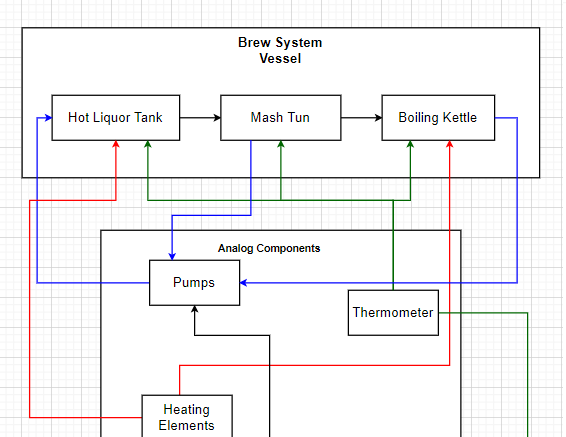
\includegraphics[width=0.60\textwidth]{images/Brew_System_Vessels}
	\caption{Brew System Vessel Layer Representation}
\end{figure}

\subsection{Hot Liquor Tank Subsystem (HLT)}
This section should be a general description of a particular subsystem for the given layer. For most subsystems, an extract of the architectural block diagram with data flows is useful. This should consist of the subsystem being described and those subsystems with which it communicates.

The main purpose of Hot Liquor Tank subsystem is to monitor and heat the water to the desired temperature. This subsystem is directly connected to three subsystems from Analog Components layer which are pumps, thermometer, and heating elements.

\subsubsection{Assumptions}
Any assumptions made in the definition of the subsystem should be listed and described. Pay particular attention to assumptions concerning interfaces and interactions with other layers.

In the initial phase, the vessel should be filled with water by the brewer. The subsystem is controlled by the micro-controller based on the current temperature of the water measured from thermometer and sent through micro-controller to the user.

\subsubsection{Responsibilities}
Each of the responsibilities/features/functions/services of the subsystem as identified in the architectural summary must be expanded to more detailed responsibilities. These responsibilities form the basis for the identification of the finer-grained responsibilities of the layer's internal subsystems. Clearly describe what each subsystem does.

The Hot Liquor Tank subsystem is responsible for providing informations such as current temperature of the water to the brewer, current status of pump and heating elements. Then the subsystem should heat the water to the desired temperature as per the brewer wants. When the water is reached to desired temperature, then it is responsible to pass the water to the Mash Tun subsystem.

\subsubsection{Subsystem Interfaces}
Each of the inputs and outputs for the subsystem are defined here. Create a table with an entry for each labeled interface that connects to this subsystem. For each entry, describe any incoming and outgoing data elements will pass through this interface.

\begin {table}[H]
\caption {Hot Liquor Tank Subsystem interfaces} 
\begin{center}
    \begin{tabular}{| p{0.75cm} | p{6cm} | p{4cm} | p{4cm} |}
    \hline
    ID & Description & Inputs & Outputs \\ \hline
    \#01 & Thermometer Subsystem & \pbox{4cm}{User input to display temperature} & \pbox{4cm}{Current Temperature of the water}  \\ \hline
    \#02 & Pump Subsystem & \pbox{4cm}{User input collected from the micro controller} & \pbox{4cm}{Open/Close the pump based on the input}  \\ \hline
    \#03 & Heating Element Subsystem & \pbox{4cm}{User input in temperature collected from the micro controller} & \pbox{4cm}{Turn on/off heating elements in order to reach user desired temperature }  \\ \hline
    \end{tabular}
\end{center}
\end{table}

\subsection{Mash Tun Subsystem}
The main purpose of Mash Tun subsystem is to mix the hot water with grains to produce wort. This subsystem is directly connected to Thermometer and Pump subsystems from Analog Components layer which is used to provide temperature of the mash.

\subsubsection{Assumptions}
When the Mash Tun is filled with hot water from the HLT, then the Mash Tun is manually loaded with the crushed grains. The user is supposed to set the temperature and time through web or app interface he want the mash to be in this subsystem. If the temperature inside the Mash Tun reached to the different temperature than the user set, the water is sent back to HLT and heated. The mash is rinse several time to rinse the sugar from the mash which is then passed to Boiling Kettle subsystem.


\subsubsection{Responsibilities}
The Mash Tun is responsible to remove sugars, mostly maltose, sucrose and maltotriose from the crushed grains to produce the final product called wort, also known as un-fermented beer. The Mash Tun should provide temperature of the current mash to the brewer. The Mash Tun is responsible to pump out the water to HLT Subsystem when it doesn't maintain required temperature. And when the water is heated enough, then it is again passed to Mash Tun subsystem. By this way, the mash is rinse to get the sugars out. The wort obtained is then passed to Boiling Kettle subsystem in this layer. 

\subsubsection{Subsystem Interfaces}
\begin {table}[H]
\caption {Mash Tun Subsystem interfaces} 
\begin{center}
	\begin{tabular}{| p{0.75cm} | p{6cm} | p{4cm} | p{4cm} |}
		\hline
		ID & Description & Inputs & Outputs \\ \hline
		\#01 & Thermometer Subsystem & \pbox{4cm}{User input to display and set temperature} & \pbox{4cm}{Current Temperature of the mash}  \\ \hline
		\#02 & Pump Subsystem & \pbox{4cm}{User input collected from the micro controller} & \pbox{4cm}{Open/Close the pump based on the temperature of the mash}  \\ \hline
	\end{tabular}
\end{center}
\end{table}

\subsection{Boiling Kettle Subsystem}
The main purpose of Boiling Kettle subsystem is to boil wort for the required amount of time. This subsystem is directly connected to Thermometer, Pump, and Heating elements subsystems from Analog Components layer which is used to maintain the amount of heat provided to the wort.

\subsubsection{Assumptions}
The Boiling Kettle subsystem is almost an automated process. The brewer have to add some hops after each beer cycle in the wort as needed because it add bitterness to the beer. The brewer must be careful with adding appropriate amount of hops as too much can ruin the taste and very little won't bring any taste to beer. 

\subsubsection{Responsibilities}
The Boiling Kettle is only responsible for heating the wort with appropriate heat for the appropriate amount of time. The wort should be heated properly to maintain the good flavor of beer. Once the boil is done, the Boiling Kettle subsystem is responsible for sending beer to the chiller for fermentation.

\subsubsection{Subsystem Interfaces}
\begin {table}[H]
\caption {Boiling Kettle Subsystem interfaces} 
\begin{center}
	\begin{tabular}{| p{0.75cm} | p{6cm} | p{4cm} | p{4cm} |}
		\hline
		ID & Description & Inputs & Outputs \\ \hline
		\#01 & Thermometer Subsystem & \pbox{4cm}{User input to display temperature} & \pbox{4cm}{Current Temperature of the wort}  \\ \hline
		\#02 & Pump Subsystem & \pbox{4cm}{User input collected from the micro controller} & \pbox{4cm}{Open/Close the pump based on the input}  \\ \hline
		\#03 & Heating Element Subsystem & \pbox{4cm}{User input in temperature collected from the micro controller} & \pbox{4cm}{Turn on/off heating elements in order to reach user desired temperature }  \\ \hline
	\end{tabular}
\end{center}
\end{table}

